\section{Mobile Platform Security}
All concepts and issued discussed below are in Android, but may also apply to iOS or other mobile OSs. 
\subsection{Mobile OS Security}
\subsubsection{Basics}
\textbf{Permission-based} access control is key design decision for Android.
Each app has private storage, own process and no communication to other apps (default). If security sensitive operation is required use \textbf{syscall} or \textbf{Android Binders}.

Each app has a designated UID.

\subsubsection{Android Binders}
Allows IPC and RPC (Remote Procedure Call).\\
Example: Accessing location goes through binder which creates channel between unprivileged app and privileged process in application framework.\\
Whether an app can use/call a binder is checked upon invocation based on the requested and granted permissions of an app.
\subsubsection{Permissions}
Three categories of permissions:\vspace{-1.5mm}
\begin{description}
    \item[normal] granted during install by default
    \item[dangerous] prompt user during runtime
    \item[signature] granted during install if signature matches signature of app which declared this permission
    \item[special] must be declared in manifest and granted by user (e.g. system overlays)
\end{description}

Android implements two reference monitors in different places:
\begin{description}
    \item[App-Framework] for system APIs
    \item[Linux-Kernel] for IPC calls to other apps
\end{description}

Problem with permission based design is twofold:
\begin{enumerate}
    \item Users can't associate privacy risks with permissions
    \item Developers tend to request too many permissions
    \item Developers fail to protect IPC interfaces (confused deputy attack)
\end{enumerate}

\subsubsection{Lessons Learned Android}
\begin{itemize}
    \item permissions concept failed in practice
    \item MAC for Android can help with privilege separation! Research required
    \item standard web technology for apps goods if sandboxed on platform
    \item further simplify APIs
    \item centralise SW distribution to protect against malicious apps
    \item vendor customization causes fragmentation and hinders updates
\end{itemize}

\subsection{Mobile Hardware Security}
\subsubsection{Trust anchors}
\begin{enumerate}
    \item platform integrity
    \item isolated execution and secure storage
    \item device authentication and remote attestation
\end{enumerate}

\begin{center}
    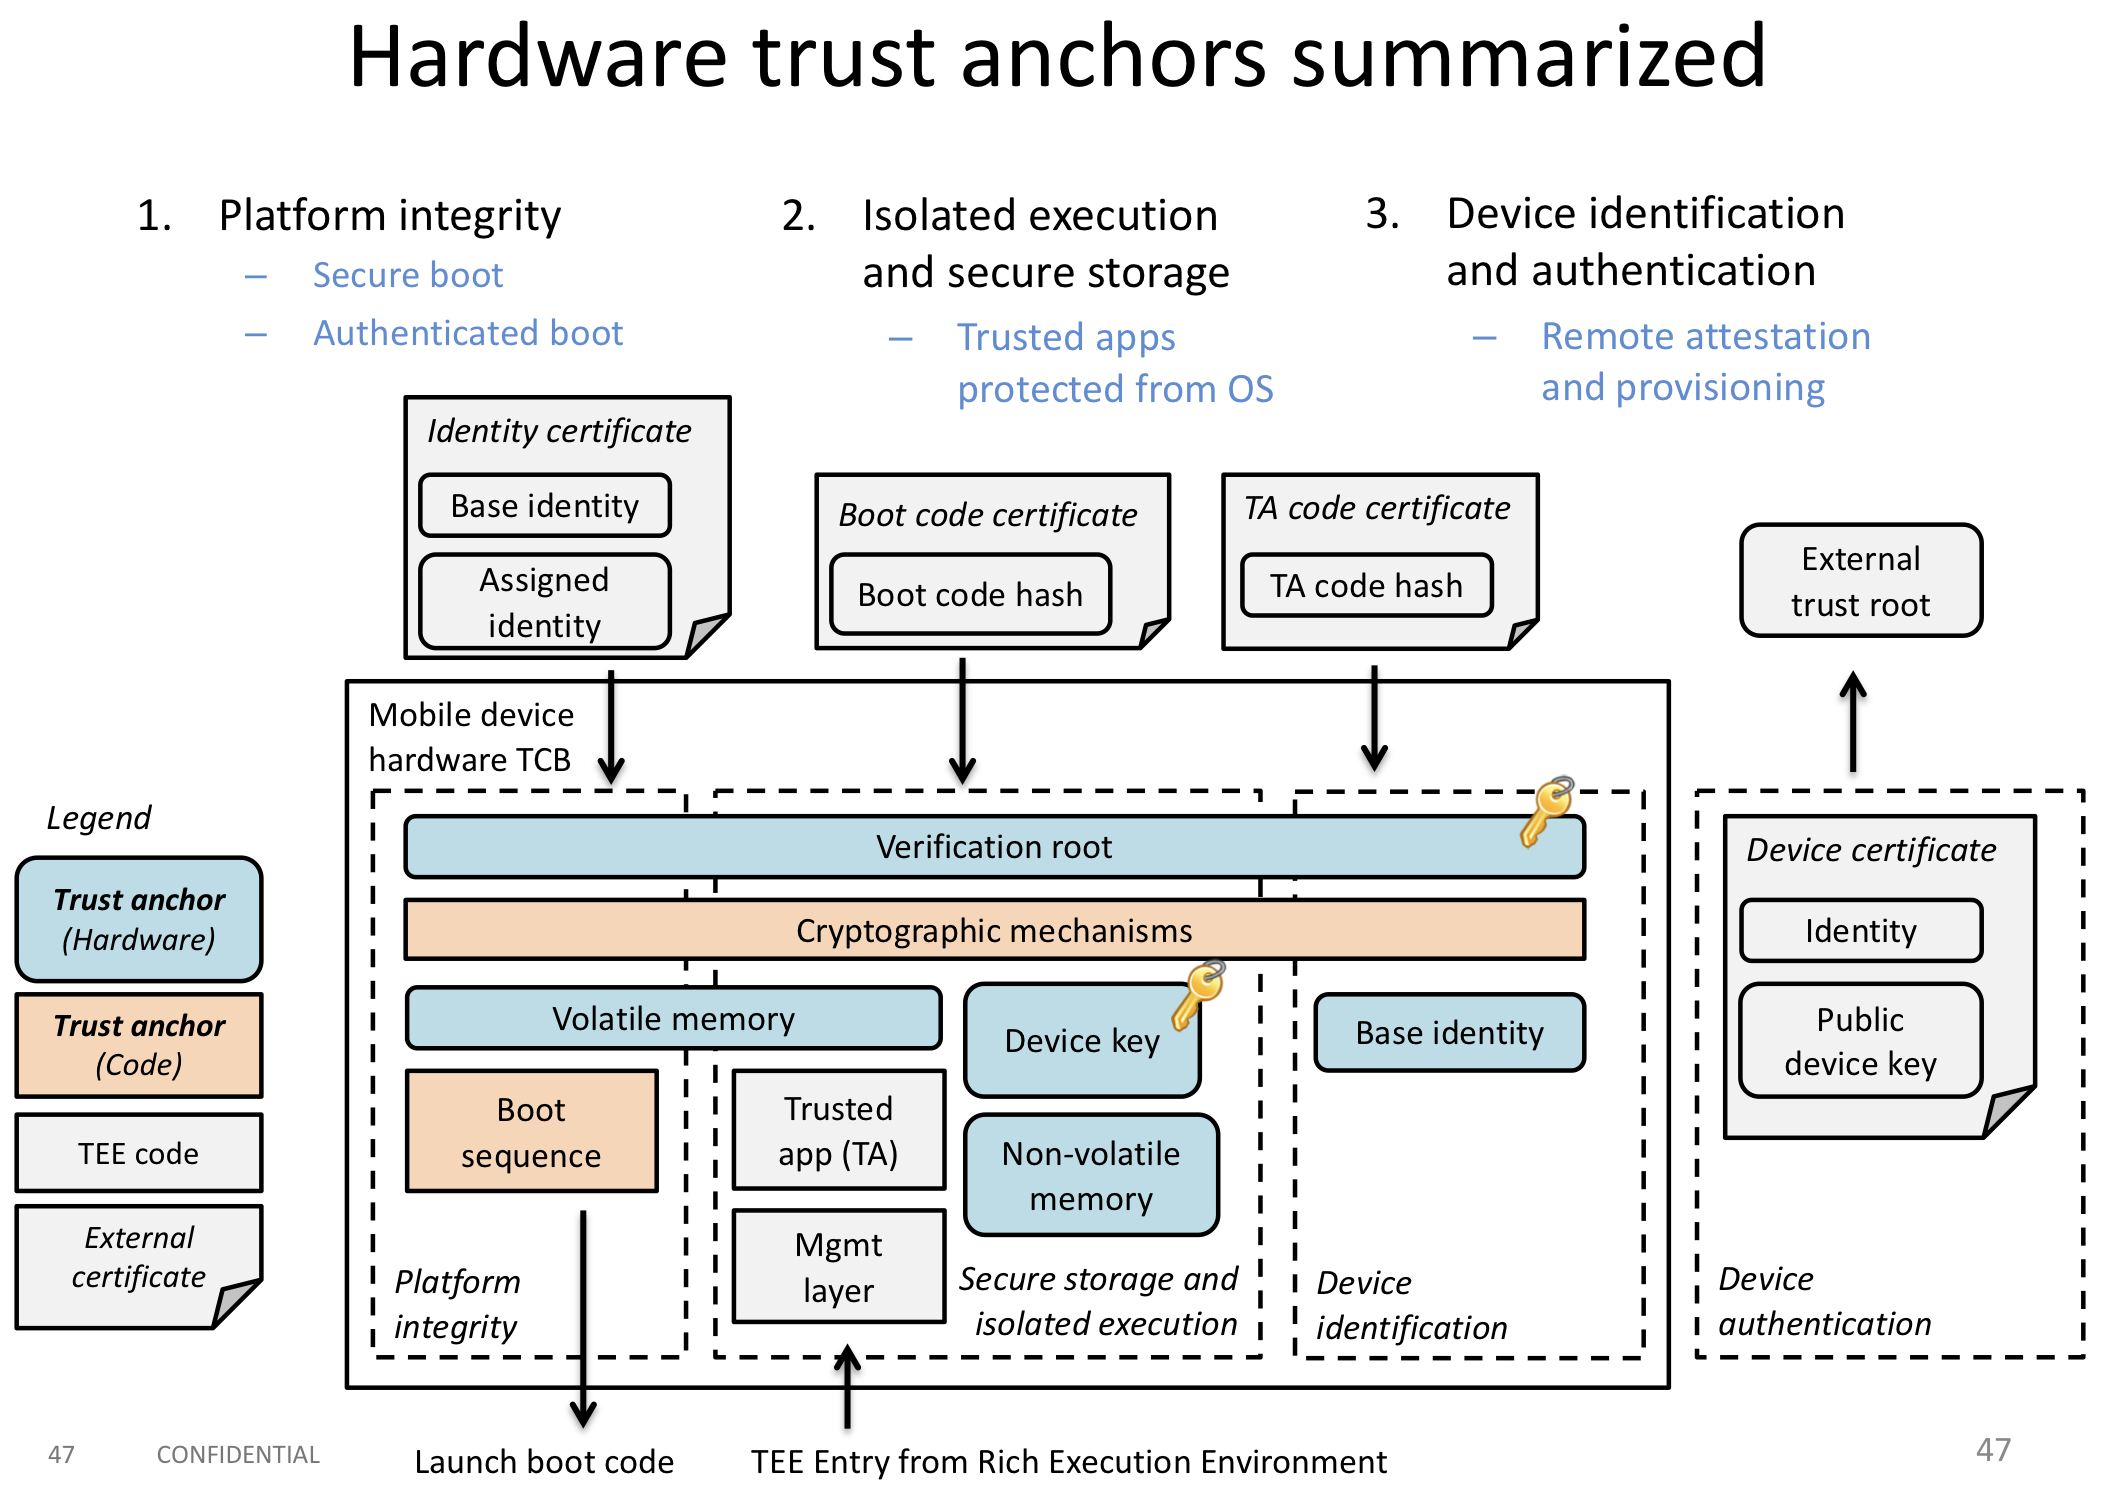
\includegraphics[width=0.85\linewidth]{images/mobile_sec_HardwareTrustAnchors.png}
\end{center}

\subsubsection{TrustZone}
TrustZone apps share the same execution environment. Therefor they mutual trust each other \textbf{or} are isolated by trusted code (TEE management layer).

TrustZone does not specify remote attestation.

App development not open.

TrustZone enables secure communication with external resources (via status flag on bus).

\begin{center}
    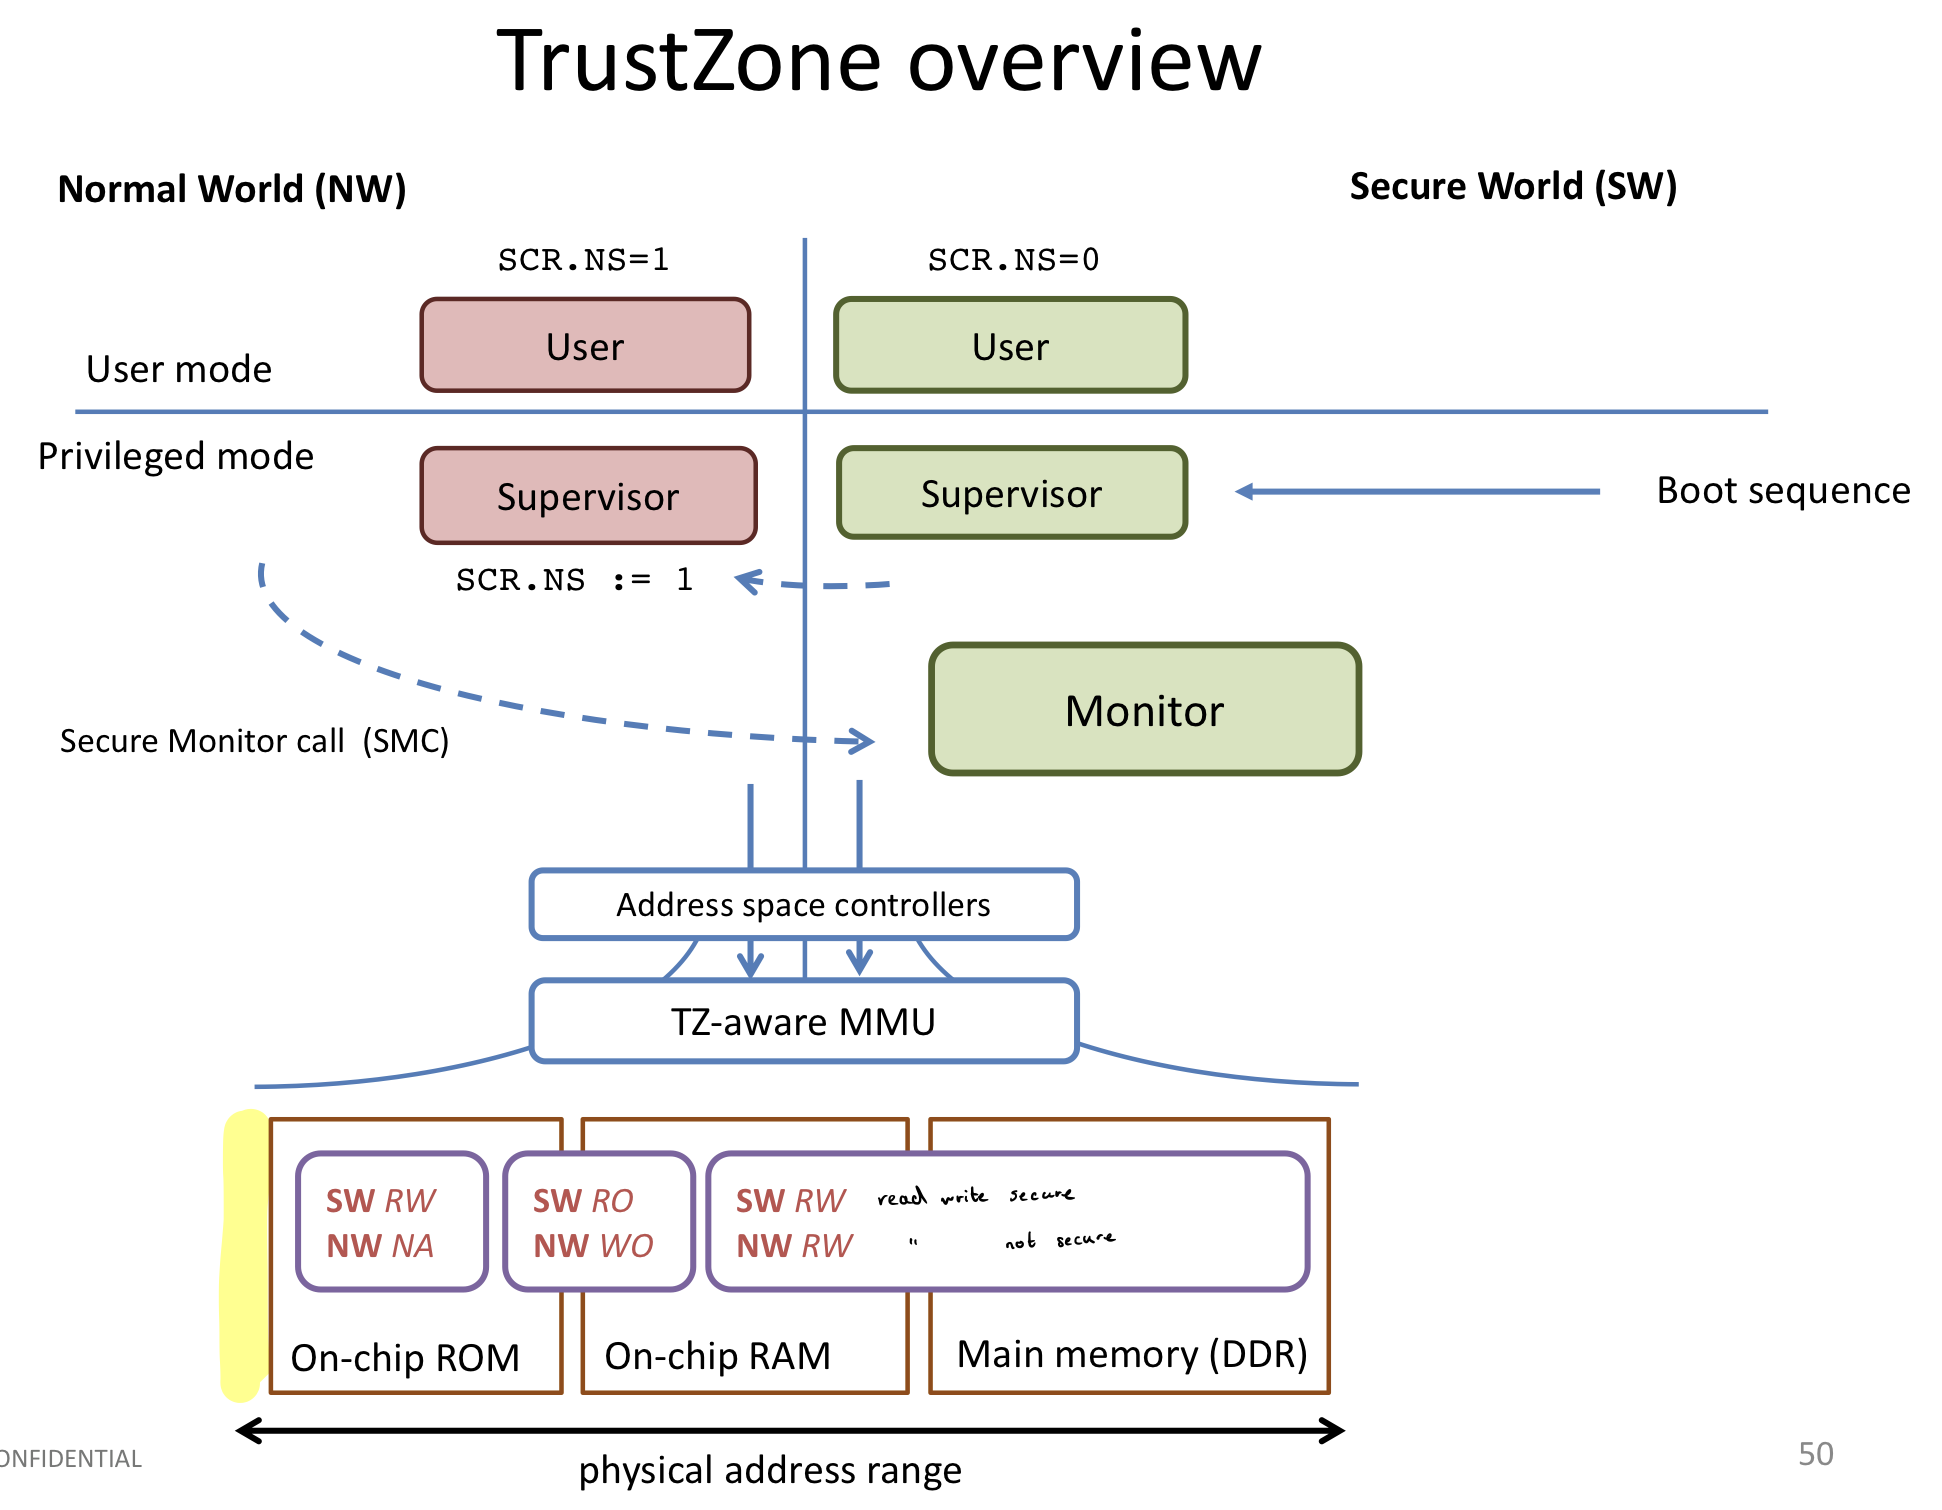
\includegraphics[width=0.8\linewidth]{images/mobile_sec_TrustZoneOverview.png}
\end{center}

Possible attacks against TrustZone: \vspace{-1.5mm}
\begin{itemize}
    \item side-channel similar to meltdown
    \item glitch attacks (e.g. PlunderVolt)
    \item replay attacks (e.g. NAND mirroring)
\end{itemize}